\documentclass{article}
\usepackage{graphicx}
\usepackage[margin=1.5cm]{geometry}
\usepackage{amsmath}

\begin{document}
\twocolumn

\title{Wednesday Warm Up: Unit 6: Fixed axis rotation}
\author{Prof. Jordan C. Hanson}

\maketitle

\section{Memory Bank}

\begin{itemize}
\item $\vec{s} = \vec{\theta} \times \vec{r}$ ... Angular displacement, arc length, and radius.
\item $\vec{v} = \vec{\omega} \times \vec{r}$ ... Angular velocity, tangential velocity,  and radius.
\item $F_{\rm C} = mr\omega^2$ ... Magnitude of centripetal force, given $\omega$.
\item $\hat{i} \times \hat{j} = \hat{k}$, $\hat{k} \times \hat{i} = \hat{j}$, $\hat{j} \times \hat{k} = \hat{i}$
\item $\hat{j} \times \hat{i} = -\hat{k}$, $\hat{i} \times \hat{k} = -\hat{j}$, $\hat{k} \times \hat{j} = -\hat{i}$
\item $\hat{i} \times \hat{i} = 0$, $\hat{j} \times \hat{j} = 0$, $\hat{k} \times \hat{k} = 0$
\item $\vec{\tau} = \vec{r} \times \vec{F}$ ... The relationship between \textit{torque}, $\vec{\tau}$, the \textit{moment arm}, $\vec{r}$, and the \textit{force}, $\vec{F}$.
\end{itemize}

\section{Fixed Axis Rotation, and Torque}

\begin{enumerate}
\item Suppose a vehicle takes a circular turn with $\vec{v} = 90\hat{j}$ km hr$^{-1}$.  (a) If $\vec{r} = 110\hat{i}$ m, what is $\vec{\omega}$? (b) If $\vec{\omega} \rightarrow 2\vec{\theta}$, but $\vec{r}$ remains constant, what is $\vec{v}$? \\ \vspace{2cm}
\item Suppose a jet fighter complex a 180 degree turn in 15 seconds, with a turn radius of 1500 m. (a) What is the tangential velocity? (b) Suppose the motion circles the origin in the xy-plane.  What is $\omega$? (c) If the jet fighter weighs 19,500 kg.  What is $F_{\rm C}$?  \\ \vspace{2cm}
\item Suppose a bolt needs to be unstuck from a flat bulkhead.  Let the bolt be centered at the origin, and let the xy-plane represent the bulkhead.  We must twist it \textit{counterclockwise} to loosen it.  (a) Suppose we have a wrench with length $\vec{r} = 5\hat{i} + 5\hat{j}$ cm attached to the bolt.  If we push on the end of the wrench with $\vec{F} = -10\hat{i}+10\hat{j}$ N of force, what is the \textit{torque} we generate? (b) Why, physically, does the torque vector have the direction we find? (c) If our wrench were longer, would that make it easier or harder to loosen the bolt? \\ \vspace{2cm}
\item Consider the balanced system in Fig. \ref{fig:1}.  (a) Qualitatively, why does this system remain stationary? (b) Calculate the torque due to the mass on the right, assuming some distance from the natural origin.  (b) Show that this torque is cancelled by the torque caused by the mass on the left.
\end{enumerate}

\begin{figure}
\centering
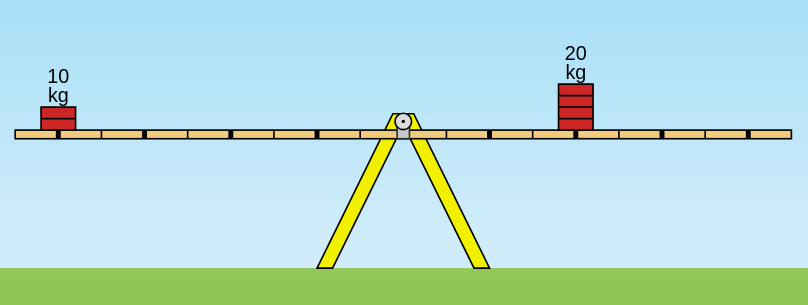
\includegraphics[width=0.4\textwidth]{figures/brick.png}
\caption{\label{fig:1} A balance between bricks of different masses.}
\end{figure}

\end{document}
